\documentclass[conference]{IEEEtran}
\IEEEoverridecommandlockouts
% The preceding line is only needed to identify funding in the first footnote. If that is unneeded, please comment it out.
\usepackage{cite}
\usepackage{amsmath,amssymb,amsfonts}
%\usepackage{algorithmic}
\usepackage{algorithm}
\usepackage{algpseudocode} % 更好控制语法结构
\usepackage{graphicx}
\usepackage{textcomp}
\usepackage{xcolor}
\usepackage{tabularx}
\usepackage{epstopdf}
\usepackage{pifont}
\usepackage{makecell}
\usepackage{hyperref}
\usepackage{enumitem}

\hypersetup{
   hypertex=true,
   colorlinks=true,
   linkcolor=blue,
   anchorcolor=blue,
   citecolor=blue
}
\setlength{\abovecaptionskip}{3pt}
\setlength{\textfloatsep}{6pt plus 1pt minus 1pt}

\def\BibTeX{{\rm B\kern-.05em{\sc i\kern-.025em b}\kern-.08em
    T\kern-.1667em\lower.7ex\hbox{E}\kern-.125emX}}
\begin{document}

\title{Mode-Adaptive Control of DC--DC Converters via Action-Regularized PPO-Based Reinforcement Learning\\}

\author{
    \IEEEauthorblockN{Chuanchuan Liang, Chaohong Zhang, Xueyong Zhang, and Weifeng Sun}
    \IEEEauthorblockA{
        Department of Integrated Circuits, Southeast University\\Nanjing 210096, China\\
        Email: \{230240065, 230258719, xueyong.zhang, swffrog\}@seu.edu.cn
    }
}

% \author{\IEEEauthorblockN{Chuanchuan Liang}
% \IEEEauthorblockA{\textit{Department of Integrated Circuits} \\
% \textit{Southeast University}\\
% Nanjing, Jiangsu, China \\
% 230240065@seu.edu.cn}

% \and
% \IEEEauthorblockN{Xueyong Zhang}
% \IEEEauthorblockA{\textit{Department of Integrated Circuits} \\
% \textit{Southeast University}\\
% Nanjing, Jiangsu, China \\
% xueyong.zhang@seu.edu.cn}
% \and
% \IEEEauthorblockN{Weifeng Sun}
% \IEEEauthorblockA{\textit{Department of Integrated Circuits} \\
% \textit{Southeast University}\\
% Nanjing, Jiangsu, China \\
% swffrog@seu.edu.cn}}

\maketitle

\begin{abstract}
DC--DC converters are fundamental in modern power electronic systems, yet their performance often deteriorates under nonlinear dynamics, parameter variations, and conduction-mode transitions, particularly when supplying constant power loads with negative impedance. Conventional controllers rely on precise models and exhibit limited robustness, while existing deep reinforcement learning (DRL) methods often suffer from oscillations and poor generalization. This paper presents a model-free control framework based on the Proximal Policy Optimization (PPO) algorithm, which expands the observation space, shapes the reward for voltage accuracy and smooth action behavior, and unifies operation across conduction modes without explicit mode detection. Trained and validated in a high-fidelity MATLAB/Simulink environment, the proposed controller achieves overshoot below \textbf{5\%}, a \textbf{10\,\textmu s} settling time, and about \textbf{4\,mV} output ripple while maintaining stability under \textbf{±30\%} parameter variations. A feasibility analysis on a \textbf{500\,MHz} Zynq-7030 FPGA shows that the trained PPO agent (two 128-neuron layers) executes approximately \textbf{1.8×10\textsuperscript{4}} MACs per inference with an estimated latency of \textbf{0.14\,\textmu s}, indicating that direct \textbf{2\,MHz} real-time control is theoretically achievable.


\end{abstract}

\begin{IEEEkeywords}
DC–DC converters, deep reinforcement learning, Proximal Policy Optimization, mode transition, action regularization
\end{IEEEkeywords}

\section{Introduction}

DC--DC converters are vital in modern power electronic systems for voltage regulation in electric vehicles, aerospace power units, and renewable energy interfaces. Their performance, however, often degrades under nonlinear dynamics, parameter variations, and conduction-mode transitions, especially when driving constant power loads with negative impedance. These effects lead to instability and poor transient response, particularly in electric vehicle DC buses and renewable energy converters, where rapid load transients demand adaptive, model-free control.

Conventional control methods such as proportional integral derivative (PID), sliding mode control (SMC), and model predictive control (MPC) depend on accurate system models and small-signal linearization. While effective under near nominal conditions, these methods face difficulties when the converter dynamics deviate from the assumed model, as establishing and maintaining model accuracy is challenging for high-frequency, time-varying systems~\cite{cui2021voltage}. To alleviate this dependence, model-free schemes using neural networks and fuzzy logic have been explored~\cite{zhao2020overview,benachour2024generalized}. Although neural networks offer strong nonlinear approximation and adaptation, their performance degrades outside the training domain, while fuzzy controllers lack generalization under rapidly changing conditions. These limitations motivate data-driven approaches that can learn optimal actions directly from converter interaction, where deep reinforcement learning (DRL) provides a promising solution.


Recent advances in DRL have demonstrated the capability to regulate nonlinear converters without explicit modeling~\cite{gheisarnejad2020iot,feng2024deep}. Algorithms such as DDPG, TD3, and DQN have shown encouraging results~\cite{tang2021artificial,ye2024td3,muktiadji2024twin,kishore2022performance}, yet often suffer from unstable convergence and excessive action oscillations that increase switching stress~\cite{min2022voltage,ye2024deep}. The Proximal Policy Optimization (PPO) algorithm mitigates these issues by constraining policy updates via a clipped objective, improving stability and control smoothness. These advantages make PPO well suited for converter control and embedded deployment.

In this work, an action-regularized PPO-based controller is developed for the DC--DC converter regulation. The framework integrates physical modeling knowledge with data-driven policy optimization to achieve robust, model-free voltage control. The main contributions are summarized as follows: 
\begin{enumerate}[leftmargin=6pt, itemsep=0pt, topsep=0pt]
    \item \textbf{Physics-informed PPO:} Embeds converter dynamics for fast transients and precise regulation.  
    \item \textbf{Reward–action co-design:} Shapes voltage error and smooths actions for stable, low-ripple switching.  
    \item \textbf{Robustness validation:} Demonstrates adaptability under mode transitions and $\pm30\%$ parameter variations.  
    \item \textbf{FPGA feasibility:} Analyzes a 500\,MHz Zynq-7030 FPGA with $\sim1.8\times10^{4}$ Multiply–Accumulate operations (MACs) per inference and 0.14\,\textmu s latency, confirming real-time 2\,MHz control feasibility.
\end{enumerate}





These contributions outline a scalable and hardware-compatible approach for intelligent, model-free converter control.

%The proposed controller is trained and tested on a high-fidelity switching model of the converter. Extensive simulation results demonstrate improved voltage regulation, enhanced dynamic response, and superior robustness against parameter uncertainties, in comparison to traditional PI-based controllers~\cite{pi_vs_drl}.


\section{System Model and Reinforcement Learning Framework}

This section introduces the dynamic model of the buck converter used for controller training and evaluation, followed by a concise overview of the PPO algorithm forming the basis of the proposed control strategy.

\subsection{System Model}

The buck converter used in this work is illustrated in Fig.~\ref{fig:buck_model}. The ideal topology is shown in Fig.~\ref{fig:buck_model}(a), while Fig.~\ref{fig:buck_model}(b) includes parasitic elements such as inductor resistance $R_L$, capacitor resistance $R_C$, switch on-resistance $R_{\text{on}}$, and diode forward drop $V_D$. The converter alternates between ON and OFF states each switching cycle, forming a hybrid nonlinear system governed by discontinuous dynamics. A high-fidelity switching model is developed to capture fast transient behavior and serves as the simulation environment for DRL training, ensuring realistic policy optimization.


%In this study, the converter is modeled in MATLAB/Simulink using a detailed switching model. The PPO agent interacts with the environment through a duty-cycle signal that is translated into a PWM signal to control the switching transistor. The environment returns observable states, including output voltage and inductor current, at each control step. This closed-loop interaction forms the training setup for the model-free control policy.




%\subsection{Conventional Control Method}

%To provide a performance benchmark, a conventional double-loop PI control strategy is implemented for the buck converter. This method is widely adopted in industrial applications due to its simplicity and reasonable performance under nominal operating conditions.

%The control architecture consists of an outer voltage loop and an inner current loop. The outer voltage loop compares the measured output voltage $V_o(t)$ with the reference voltage $V_{\text{ref}}$ to generate a reference current $i_{\text{ref}}(t)$. The inner loop then compares $i_{\text{ref}}(t)$ with the actual inductor current $i_L(t)$ to generate the duty cycle $d(t)$, which is applied to the PWM generator.

%The control laws for the two loops are expressed as:

%\begin{equation}
%\begin{aligned}
%i_{\text{ref}}(t) &= K_{pv}(V_{\text{ref}} - V_o(t)) + K_{iv} \int_0^t (V_{\text{ref}} - V_o(\tau))\,d\tau \\
%d(t) &= K_{pi}(i_{\text{ref}}(t) - i_L(t)) + K_{ii} \int_0^t (i_{\text{ref}}(\tau) - i_L(\tau))\,d\tau
%\end{aligned}
%\end{equation}

%where $K_{pv}$ and $K_{iv}$ are the proportional and integral gains for the voltage loop, and $K_{pi}$ and $K_{ii}$ are the corresponding gains for the current loop.

%hile the double-loop PI controller achieves satisfactory performance under steady-state conditions, its effectiveness degrades in the presence of parameter perturbations or conduction mode transitions. Specifically, fixed-gain PI controllers are not inherently robust to variations in inductance, capacitance, or load resistance, and may require manual retuning. Furthermore, abrupt changes in control signals can induce overshoot, oscillations, or increased switching losses, which limits their applicability in scenarios with high dynamic uncertainty.

%This motivates the adoption of a model-free control approach capable of adapting to nonlinear dynamics and operating uncertainties without explicit system modeling or manual parameter tuning.
%The block diagram of conventional double-loop PI is shown in Fig. 2.

\subsection{Deep Reinforcement Learning}

DRL enables model-free control through agent–environment interaction guided by scalar rewards. For converter regulation, the underlying algorithm must support model-free operation, robust convergence, and high sample efficiency~\cite{mazaheri2024deep}. As summarized in Table~\ref{tab:DRLcompare}, the PPO algorithm  offers stable convergence and efficient policy learning via its clipped surrogate objective:

\begin{figure}[b]
  \centering
  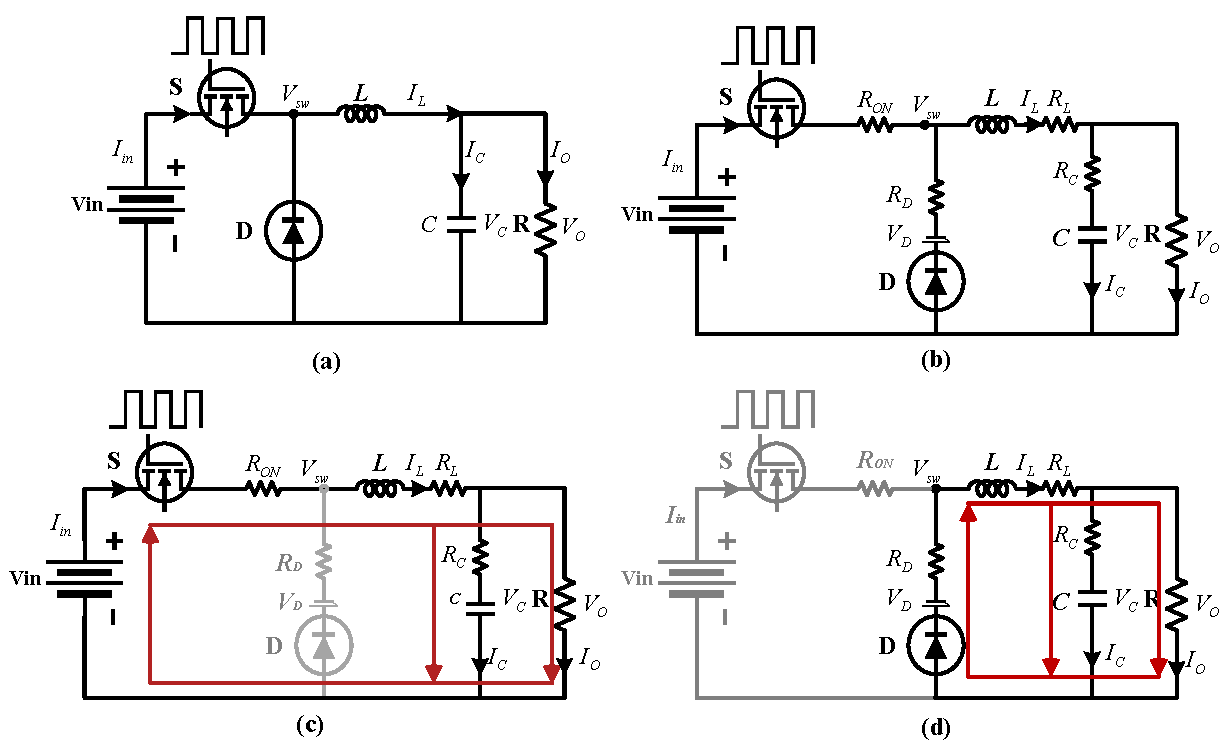
\includegraphics[width=0.48\textwidth]{figs/buck_model5.pdf}
  \caption{(a) Ideal buck converter; (b) Non-ideal converter with parasitic components; (c) ON-state equivalent circuit; (d) OFF-state equivalent circuit.}
  \label{fig:buck_model}
\end{figure}


% 替代对勾符号
\newcommand{\cmark}{\ding{51}} % 对勾
\newcommand{\xmark}{\ding{55}} % 叉号

% \begin{table*}[t]
% \centering
% \caption{Comparison of DRL algorithms for converter control.}
% \label{tab:DRLcompare}
% \begin{tabular}{lccccc}
% \hline\hline
% \textbf{Algorithm Type} & 
% \makecell[c]{\textbf{No Model} \\ \textbf{Required}} & 
% \makecell[c]{\textbf{Sample \&} \\ \textbf{Computation Efficient}} & 
% \makecell[c]{\textbf{Hyperparameter} \\ \textbf{Robustness}} & 
% \makecell[c]{\textbf{Continuous} \\ \textbf{Action Support}} \\
% \hline
% \textbf{Model-Free} &  &   &   &   \\
% Value-Based (e.g., DQN)       & \cmark & \cmark & \cmark & \xmark \\
% Policy-Based (e.g., PG)       & \cmark & \xmark & \xmark & \cmark \\
% Actor–Critic (e.g., PPO) & \cmark & \cmark\cmark\cmark & \cmark\cmark\cmark & \cmark \\
% Actor–Critic (e.g., TD3) & \cmark & \cmark\cmark & \cmark\cmark & \cmark \\
% Actor–Critic (e.g., DDPG) & \cmark & \cmark & \cmark & \cmark \\
% \hline
% \textbf{Model-Based}                               & \xmark & \cmark\cmark & \cmark\cmark & \cmark \\
% \hline
% \end{tabular}
% \end{table*}
\begin{table*}[t]
\centering
\caption{Comparison of representative DRL algorithms for DC--DC converter control.}
\label{tab:DRLcompare}
\begin{tabular}{lcccc}
\hline\hline
\textbf{Algorithm} & 
\textbf{Sample \& Computation Efficiency} & 
\textbf{Hyperparameter Robustness} & 
\textbf{Continuous Action Support} & 
\textbf{Model Requirement} \\
\hline
\textbf{Model-Free} &  &   &   &   \\
Value-Based (e.g., DQN)         & High     & High     & No      & No \\
Policy-Based (e.g., PG)         & Low      & Low      & Yes     & No \\
Actor--Critic (e.g., PPO)       & High & High & Yes     & No \\
Actor--Critic (e.g., TD3)       & Good     & Good     & Yes     & No \\
Actor--Critic (e.g., DDPG)      & Fair     & Fair     & Yes     & No \\
\hline
\textbf{Model-Based}     & Good     & Good     & Yes     & Yes \\
\hline
\end{tabular}

\end{table*}


%Traditional value-based methods such as Q-learning and DQN are restricted to discrete action spaces, making them unsuitable for high-resolution PWM control. While DDPG addresses this limitation through deterministic policies and supports continuous control, it suffers from instability during training due to Q-value overestimation. TD3 improves upon DDPG by using twin critics and delayed policy updates, enhancing convergence stability. However, TD3 can still be sensitive to hyperparameter settings and may require extensive tuning.

%Compared to these alternatives, PPO strikes a favorable balance between stability and performance. As an actor–critic algorithm, PPO combines the benefits of both policy-based and value-based approaches. It performs stable policy updates through a clipped surrogate objective, which constrains large policy deviations and reduces training oscillations. PPO also supports continuous action spaces and has been shown to offer strong robustness across various control scenarios.

\begin{equation}
L^{\text{CLIP}}(\theta) = \mathbb{E}_t \left[ \min \left( r_t(\theta) \hat{A}_t, \ \text{clip}(r_t(\theta), 1 - \epsilon, 1 + \epsilon) \hat{A}_t \right) \right]
\label{eq:ppo_clip}
\end{equation}

where $r_t(\theta) = \frac{\pi_\theta(a_t | s_t)}{\pi_{\theta_{\text{old}}}(a_t | s_t)}$ is the policy ratio between successive updates, and $\hat{A}_t$ denotes the advantage estimate. The clipping threshold $\epsilon$ (typically 0.1–0.3) constrains large updates and ensures smooth, monotonic policy improvement.


PPO adopts an actor–critic architecture, where the actor outputs discrete duty-cycle actions and the critic estimates value functions, as illustrated in Fig.~\ref{fig:PPO} and Algorithm~\ref{alg:ppo}. The framework integrates environment interaction, advantage estimation, experience replay, and actor–critic updates based on a clipped surrogate objective. By constraining policy updates and smoothing discrete actions, PPO achieves stable and robust convergence for DC--DC converter control under fast transients and nonlinear conditions.

\begin{figure}[t]
  \centering
  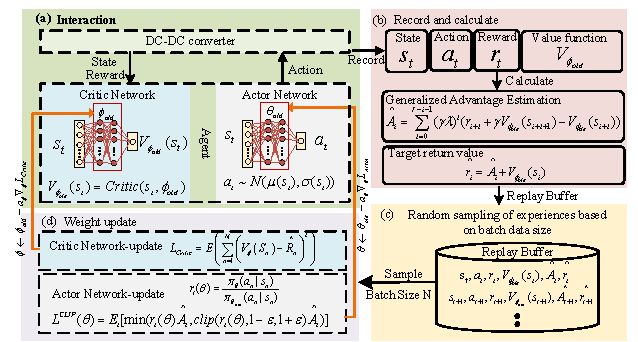
\includegraphics[width=0.48\textwidth]{figs/ppo_structure66.pdf}
  \caption{Architecture of the PPO-based model-free control framework.}
  \label{fig:PPO}
\end{figure}

\begin{algorithm}[!t]
\caption{PPO-clipped}
\label{alg:ppo}
\begin{algorithmic}[1]
\State \textbf{Input:} Initial policy parameters $\theta_0$, initial value function parameters $\phi_0$
\For{$k = 0, 1, 2, \ldots$}
    \State Collect the set of trajectories $D_k = \{\tau_i\}$ by running the policy $\pi_k = \pi(\theta_k)$ in the environment.
    \State Compute rewards-to-go, $\hat{r}_t$, representing the cumulative sum of future rewards from time step $t$ onward.
    \State Compute advantage estimates, $\hat{A}_t$, based on the current value function $V_{\phi_k}$ which represents the expected return from a given state.
    \State Update the policy by maximizing the PPO-clip:
    \[
        \theta_{k+1} \leftarrow \arg\max_\theta L^{\text{CLIP}}(\theta)
    \]
   \State Fit value function by regression on mean-squared error:
    \[
        \phi_{k+1} \leftarrow \arg\min_\phi \frac{1}{|D_k||T|} \sum_{\tau \in D_k} \sum_{t=0}^{T} \left( V_\phi(s_t) - \hat{r}_t \right)^2
   \]
\EndFor
\end{algorithmic}
\end{algorithm}


\section{Proposed Model-Free Control}

To ensure stable and adaptive voltage regulation, the proposed framework couples the buck converter model with the PPO algorithm. The converter serves as the environment, while the PPO agent learns optimal duty-cycle actions through interaction by observing states, applying controls, and receiving rewards that quantify regulation quality. The observation, action, and reward formulations are detailed below.


\subsection{Observation Space}

The observation vector includes input voltage $V_{\text{in}}$, inductor current $i_L$, output current $i_{\text{out}}$, reference voltage $V_{\text{ref}}$, and voltage error $e = V_{\text{ref}} - V_{\text{out}}$. To embed temporal dynamics, each signal is sampled at two consecutive steps, forming a 10-dimensional observation vector:


\begin{equation}
\mathbf{obs}(t) =
\begin{bmatrix}
V_{\text{in}}(t),\ i_L(t),\ i_{\text{out}}(t),\ V_{\text{ref}}(t),\ e(t) \\
V_{\text{in}}(t{-}1),\ i_L(t{-}1),\ i_{\text{out}}(t{-}1),\ V_{\text{ref}}(t{-}1),\ e(t{-}1)
\end{bmatrix}
\label{eq:obs_vector}
\end{equation}

This design allows the PPO agent to infer system dynamics implicitly through sequential state information rather than relying on explicit physical modeling, enabling model-free learning of transient converter behavior.

\subsection{Action Space}
The PPO agent outputs discrete duty-cycle commands $a_t\!\in\!\{0,\Delta a,2\Delta a,\ldots,1\}$, 
where $\Delta a$ represents the duty-cycle step size defined by the FPGA resolution. 
At steady state, the converter output satisfies $V_{\text{out}}\!\approx\!a_tV_{\text{in}}$, 
and the corresponding relative quantization error can be approximated by
\begin{equation}
\frac{\Delta V_{\text{out}}}{V_{\text{out}}}\!\approx\!\frac{\Delta a}{a_t}.
\end{equation}
Here, $a_t$ represents the discrete duty-cycle value selected by the PPO policy at each time step. 

Under the worst-case condition ($V_{\text{in}}=8$\,V, $V_{\text{out}}=1.5$\,V), the minimum duty ratio is $a_{t,\min} = 0.1875$. 
To keep the steady-state error below 1\%, the step size must satisfy $\Delta a\!\le\!0.001875$. 
Thus, $\Delta a=1/1024\!\approx\!0.098\%$ is adopted, providing adequate precision for stable voltage regulation.


\subsection{Reward Function}
The reward function jointly improves voltage regulation accuracy and control smoothness. It combines a voltage error penalty and an action variation term, defined as:

\begin{equation}
R_t =
\begin{cases}
-k_1 \sqrt{\left| e_{\text{norm}} \right|} - k_2 \left| e_{\text{action}} \right|, & \text{if } \left| e_{\text{norm}} \right| < 0.01 \\[6pt]
-k_3 \sqrt{\left| e_{\text{norm}} \right|}, & \text{otherwise}
\end{cases}
\label{eq:reward}
\end{equation}

Here, $e_{\text{norm}} = e_t / V_{\text{ref}}$ denotes the normalized voltage error, and $e_{\text{action}} = a_t - a_{t-1}$ is the duty-cycle change. The first term promotes steady-state accuracy, while the second term serves as an action-regularization component, penalizing large temporal differences in control actions to reduce switching stress and high-frequency oscillations. 


\section{RESULTS AND DISCUSSION}

This section evaluates the proposed PPO-based controller in terms of training performance, robustness, dynamic response, reward formulation, and implementation feasibility.

\subsection{Training Performance}

The controller was trained in MATLAB/Simulink using parameters listed in Tables~\ref{tab:buck_params} and~\ref{tab:trainparams}. As shown in Fig.~\ref{fig:training_curve}, the cumulative reward increased steadily and saturated after about 300 episodes, indicating consistent policy improvement and convergence. This stable learning behavior validates the reward formulation and network design, establishing a reliable basis for performance evaluation.

\subsection{Robustness Evaluation}

Controller robustness was tested under $\pm30\%$ perturbations of inductance and capacitance. As illustrated in Fig.~\ref{fig:indcap}, output voltage deviations remained below 1\% in all cases. For inductance variations around $0.47\,\mu$H, errors ranged from $-0.62\%$ to $+0.13\%$, and for capacitance variations of $44\,\mu$F~$\pm30\%$, from $-0.19\%$ to $-0.01\%$. These results confirm strong parameter tolerance and effective policy generalization beyond the training domain.

\subsection{Dynamic Performance and Mode Transition}

Dynamic performance was assessed under abrupt changes in input voltage, load, and reference, which triggered CCM/DCM transitions (Fig.~\ref{fig:ccm_dcm}). Across all conditions, the controller maintained stable operation without oscillations or duty-cycle saturation. The output voltage tracked the reference with steady-state error within $\pm0.7\%$, overshoot under 5\%, and recovery within $10\,\mu$s after each disturbance, demonstrating fast and robust transient response.

\begin{table}[t]
\caption{Buck Converter Parameters}
\label{tab:buck_params}
\centering
\begin{tabularx}{\linewidth}{>{\centering\arraybackslash}X >{\centering\arraybackslash}X >{\centering\arraybackslash}X}
\hline\hline
\textbf{Parameter} & \textbf{Symbol} & \textbf{Value} \\
\hline
Input voltage        & $V_{\text{in}}$         & $2\,\text{V} \sim 8\,\text{V}$ \\
Reference voltage    & $V_{\text{ref}}$        & $1.5\,\text{V} \sim 5\,\text{V}$ \\
Inductance           & $L$                    & 0.47 uH         \\
Capacitance          & $C$                    & 44 uF       \\
Inductor DCR         & $R_{\text{L}}$       & 3.7 $m\Omega$  \\
Capacitor ESR        & $R_{\text{C}}$       & 3 $m\Omega$ \\
Switching frequency  & $f_{\text{sw}}$        & 2 MHz         \\
Load current         & $I_{\text{load}}$      & $0.6\,\text{A} \sim 6\,\text{A}$ \\
\hline
\end{tabularx}
\end{table}

\begin{table}[t]
\caption{Training Parameters and Hardware Configuration}
\label{tab:trainparams}
\centering
\begin{tabular}{lc}
\hline\hline
\textbf{Parameters} & \textbf{Value} \\
\hline
Agent sample time & $0.5 \times 10^{-6}$ seconds \\
Training episodes & 300 \\
Discount factor & 0.99 \\
PPO clip parameter & 0.2 \\
Neural network structure & [10, 128, 128,1] \\
Activation function & ReLU \\
$k_1$, $k_2$, $k_3$ & 10, 500, 20 \\
Size of random experience mini-batch & 512 \\
Approximate duration of training & 1 hours \\
CPU & Intel(R) Core(TM) i9-14900HX \\
     & @ 2.20\,GHz \\
RAM & 32 GB \\
\hline
\end{tabular}
\end{table}

\begin{figure}[!t]
\centering
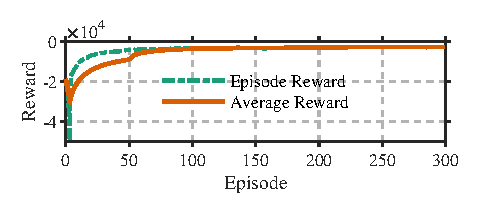
\includegraphics[width=0.8\linewidth]{figs/reward2.eps}
\caption{Training curve of the PPO-based controller over 300 episodes.}
\label{fig:training_curve}
\end{figure}

\begin{figure}[!t]
\centering
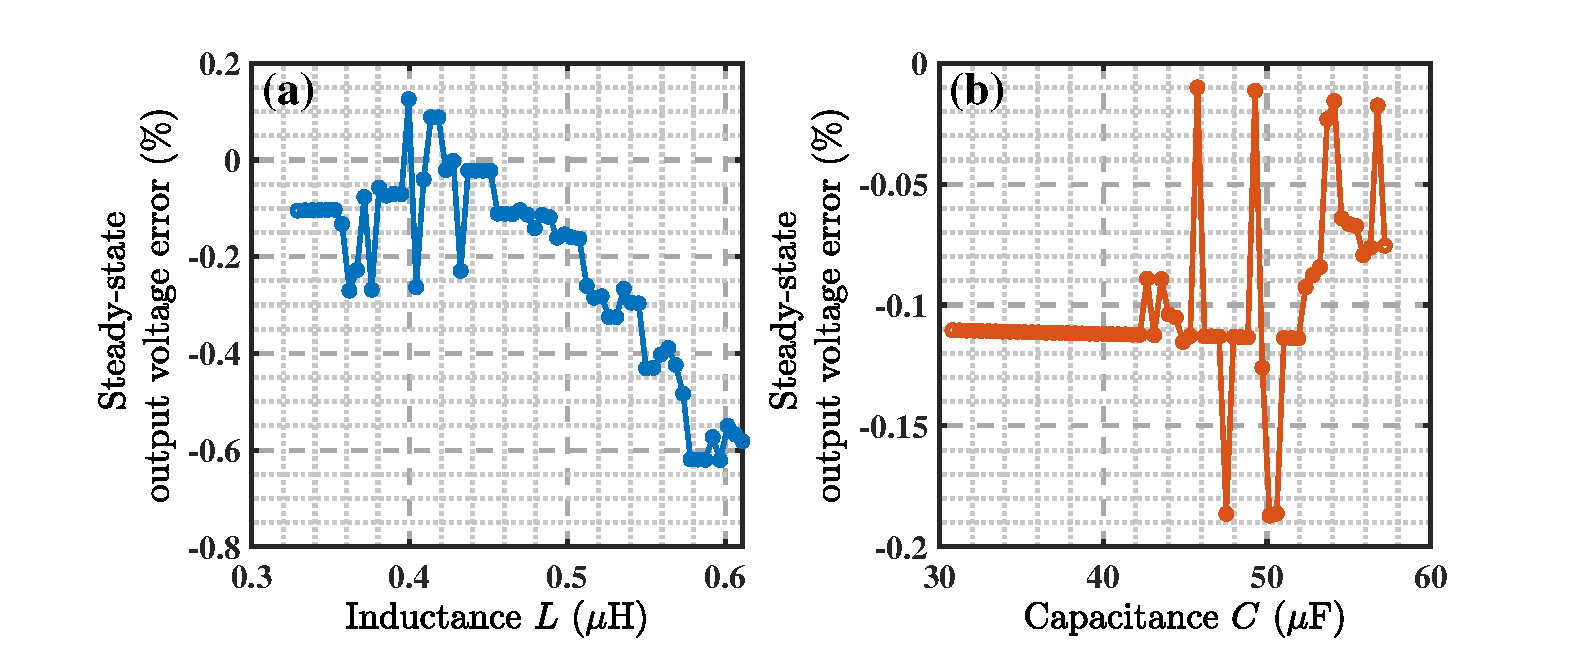
\includegraphics[width=\linewidth]{figs/indcap.eps}
\caption{Steady-state output voltage error under $\pm30\%$ uncertainty in (a) inductance ($0.47\,\mu\text{H}$) and (b) capacitance ($44\,\mu\text{F}$) parameters.}
\label{fig:indcap}
\end{figure}

\subsection{Impact of Action-Regularized Reward}

The effect of action regularization was examined at $V_{\text{in}}=4$\,V, $V_{\text{ref}}=2.2$\,V, and $I_{\text{load}}=3$\,A. Without the constraint, the duty-cycle signal exhibited high-frequency jitter with a dominant period of 10\,$\mu$s, producing $\sim$15\,mV output ripple. With the constraint applied, switching became smoother and more periodic, with a dominant period of 0.5\,$\mu$s, and the ripple reduced to $\sim$4\,mV (Fig.~\ref{fig:voltage_comparison}). This confirms that the reward design effectively suppresses switching noise and enhances steady-state precision.


\begin{figure}[!t]
    \centering
    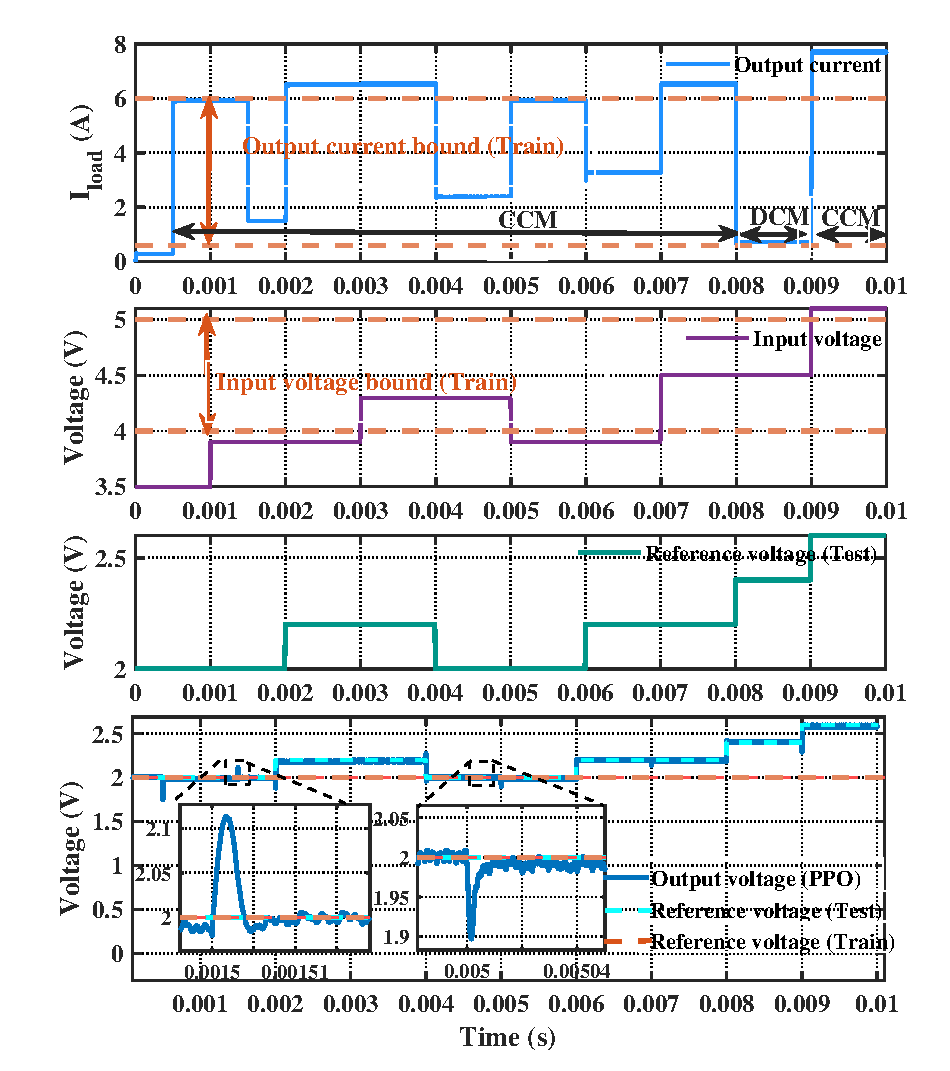
\includegraphics[width=0.95\linewidth]{figs/ccm330.eps} 

    \caption{Results of scenarios where variations in output current, input voltage, and reference voltage occur outside the training range.}
    \label{fig:ccm_dcm}
\end{figure}

\begin{figure}[!t]
\centering
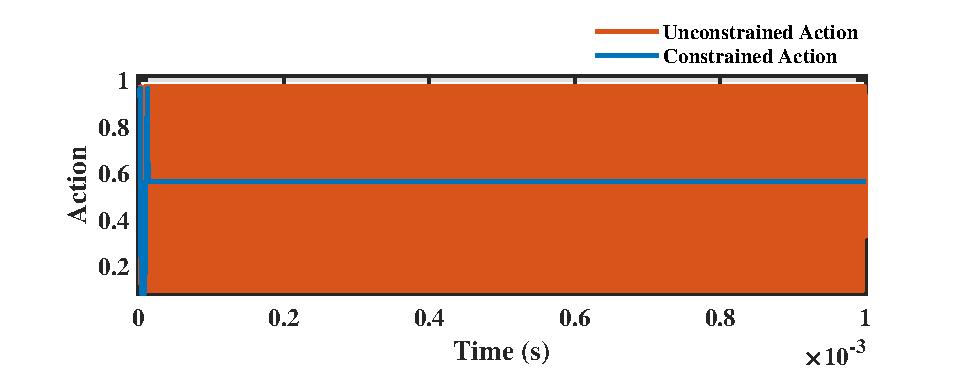
\includegraphics[width=0.48\textwidth]{figs/action_compare4.eps}
\caption{Action trajectories of the PPO-based controller under $V_{\text{in}}=4$\,V, $V_{\text{ref}}=2.2$\,V, and $I_{\text{load}}=3$\,A.}
\label{fig:action_comparison}
\end{figure}

\begin{figure}[t]
\centering
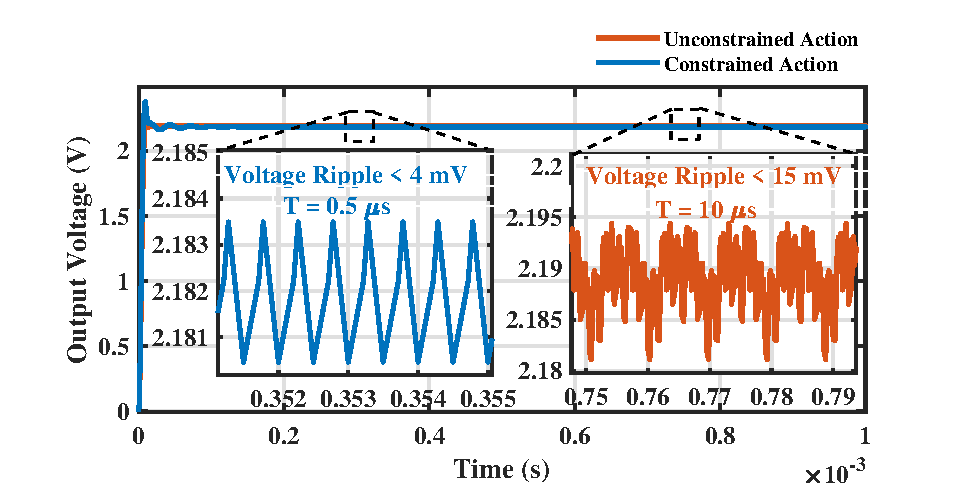
\includegraphics[width=0.48\textwidth]{figs/voltage_action_compare66.eps}
\caption{Output voltage responses under unconstrained and constrained action trajectory.}
\label{fig:voltage_comparison}
\end{figure}

\subsection{Computational Complexity and Implementation Feasibility}

The trained PPO network includes two hidden layers of 128 neurons and the total operations are approximated as:
\begin{equation}
\mathrm{MACs}=10\times128+128\times128+128\times1\approx1.8\times10^{4}
\end{equation}

The Xilinx Zynq-7030 FPGA integrates 400 DSP48E1 slices, each capable of one multiply–accumulate (MAC) per clock cycle under full pipelining. 
Assuming a clock frequency of $f_{\text{clk}}=500$\,MHz and an effective utilization of $\eta_{\text{dsp}}=0.65$ accounting for activation and control overhead, 
the achievable throughput is given by
\begin{equation}
R_{\text{eff}}=\eta_{\text{dsp}} N_{\text{DSP}} f_{\text{clk}}
\approx1.3\times10^{11}~\text{MAC/s}.
\end{equation}

Including activation and bias operations, the total inference cost is $\mathrm{MACs}_{\text{tot}}\!\approx\!1.85\times10^{4}$, and the corresponding inference latency can be estimated as $\tau_{\text{inf}}\!=\!\mathrm{MACs}_{\text{tot}}/R_{\text{eff}}\!\approx\!0.14\,\mu\text{s}$, which is well below the 0.5\,$\mu$s switching period of a 2\,MHz converter, confirming the feasibility of direct cycle-by-cycle PPO inference.


\section{Conclusions And Future Work}

This work presents a PPO-based model-free controller for DC--DC converter regulation. 
Physics-informed training and action regularization enable fast transients ($10\,\mu$s), low overshoot ($<5\%$), 
and high steady-state precision ($\pm0.7\%$). 
The trained agent, with two 128-neuron layers, performs $\sim1.8\times10^{4}$ MACs per inference 
and achieves $0.14\,\mu\text{s}$ latency on a $500\,\text{MHz}$ Zynq-7030 FPGA, 
demonstrating feasibility for direct $2\,\text{MHz}$ real-time control. 
Future work will focus on Hardware-in-the-Loop and prototype validation.


\bibliographystyle{IEEEtran}
\bibliography{references} 

\end{document}
